\documentclass{beamer}

\usepackage[utf8]{inputenc}
\usepackage{default}

\mode<presentation>
%{ \usetheme{boxes} }


\usetheme{Madrid}

\usepackage{times}
\usepackage{graphicx}
\usepackage{tabulary}
\usepackage{listings}
\usepackage{verbatimbox}
\usepackage{graphicx}
\usepackage{lmodern}
\usepackage[absolute,overlay]{textpos}
\usepackage{pgfpages}
\usepackage{color}
\usepackage{multicol}

\pgfdeclareimage[height=1.0cm]{logo_rcc}{icons/logo_rcc.png}
\setlength{\TPHorizModule}{1mm}
\setlength{\TPVertModule}{1mm}
\newcommand{\RCCLogo}{
\begin{textblock}{14}(1.5,1.5)
  \pgfuseimage{logo_rcc}
\end{textblock}
}

\pgfdeclareimage[height=1.0cm]{spark}{icons/spark.png}
\newcommand{\SPARK}{
\begin{textblock}{14}(107.5,1.5)
  \pgfuseimage{spark}
\end{textblock}
}



\definecolor{mycolorcli}{RGB}{53,154,26}
\definecolor{mycolorcode}{RGB}{0,0,255}
\definecolor{mycolordef}{RGB}{255,0,0}
\definecolor{mycolorlink}{RGB}{184,4,255}

\setcounter{tocdepth}{3}

\title{\huge{Introduction to Spark}}
\author{Igor Yakushin \\ \texttt{ivy2@uchicago.edu}}

\definecolor{ChicagoMaroon}{RGB}{128,0,0}

\setbeamercolor{title}{bg=ChicagoMaroon}

\begin{document}

\setbeamertemplate{navigation symbols}{}

\setbeamercolor{fcolor}{fg=white,bg=ChicagoMaroon}
\setbeamertemplate{footline}{
\begin{beamercolorbox}[ht=4ex,leftskip=1.4cm,rightskip=.3cm]{fcolor}
\hrule
\vspace{0.1cm}
   \hfill \insertshortdate \hfill \insertframenumber/\inserttotalframenumber
\end{beamercolorbox}
}

\setbeamercolor{frametitle}{bg=ChicagoMaroon,fg=white}

\begin{frame}
\RCCLogo
\SPARK
\titlepage
\end{frame}
\section{How to get this tutorial}
\begin{frame}[fragile]
  \frametitle{How to get this tutorial}

  \begin{itemize}
  \item Point your browser to:
    {\color{mycolorcli}
\begin{verbatim}
https://git.rcc.uchicago.edu/ivy2/Spark
\end{verbatim}
    }
  \item Once you log into midway, get the tutorial:
    {\color{mycolorcli}
\begin{verbatim}
git clone https://git.rcc.uchicago.edu/ivy2/Spark.git
cd Spark
\end{verbatim}
    }
  \item The presentation is in {\color{mycolorcli}docs/Spark.pdf}
  \item The labs are in {\color{mycolorcli}labs/}
  \end{itemize}
\end{frame}  
\section{How to login to midway}

\subsection{ssh}
\begin{frame}[fragile]
  \frametitle{Login to midway: ssh}
  \begin{itemize}
  \item {\color{mycolorcli}ssh} - {\color{mycolordef}s}ecure {\color{mycolordef}sh}ell. 
  \item {\color{mycolordef}If you have an account on midway}:
{\color{mycolorcli}
\begin{verbatim}
ssh <cnetid>@midway2.rcc.uchicago.edu
\end{verbatim}
}
  \item This assumes that you have ssh client on your laptop.
  \item If you have Mac or run Linux on your laptop, you should have it
  \item If you have MS Windows, you might need to install a client: 
    for example {\color{mycolorcli}putty} or {\color{mycolorcli}bitvise} from  {\color{mycolorcli}\verb|http://www.putty.org|}.
  \item On Chromebook or any other OS you can use ssh extention to Chrome browser.
  \end{itemize}
\end{frame}

\subsection{yubikey}
\begin{frame}[fragile]
  \frametitle{Login to midway: yubikey}
  \begin{itemize}
  \item {\color{mycolordef}If you do not have an account on midway cluster}, use {\color{mycolordef}yubikey}:
    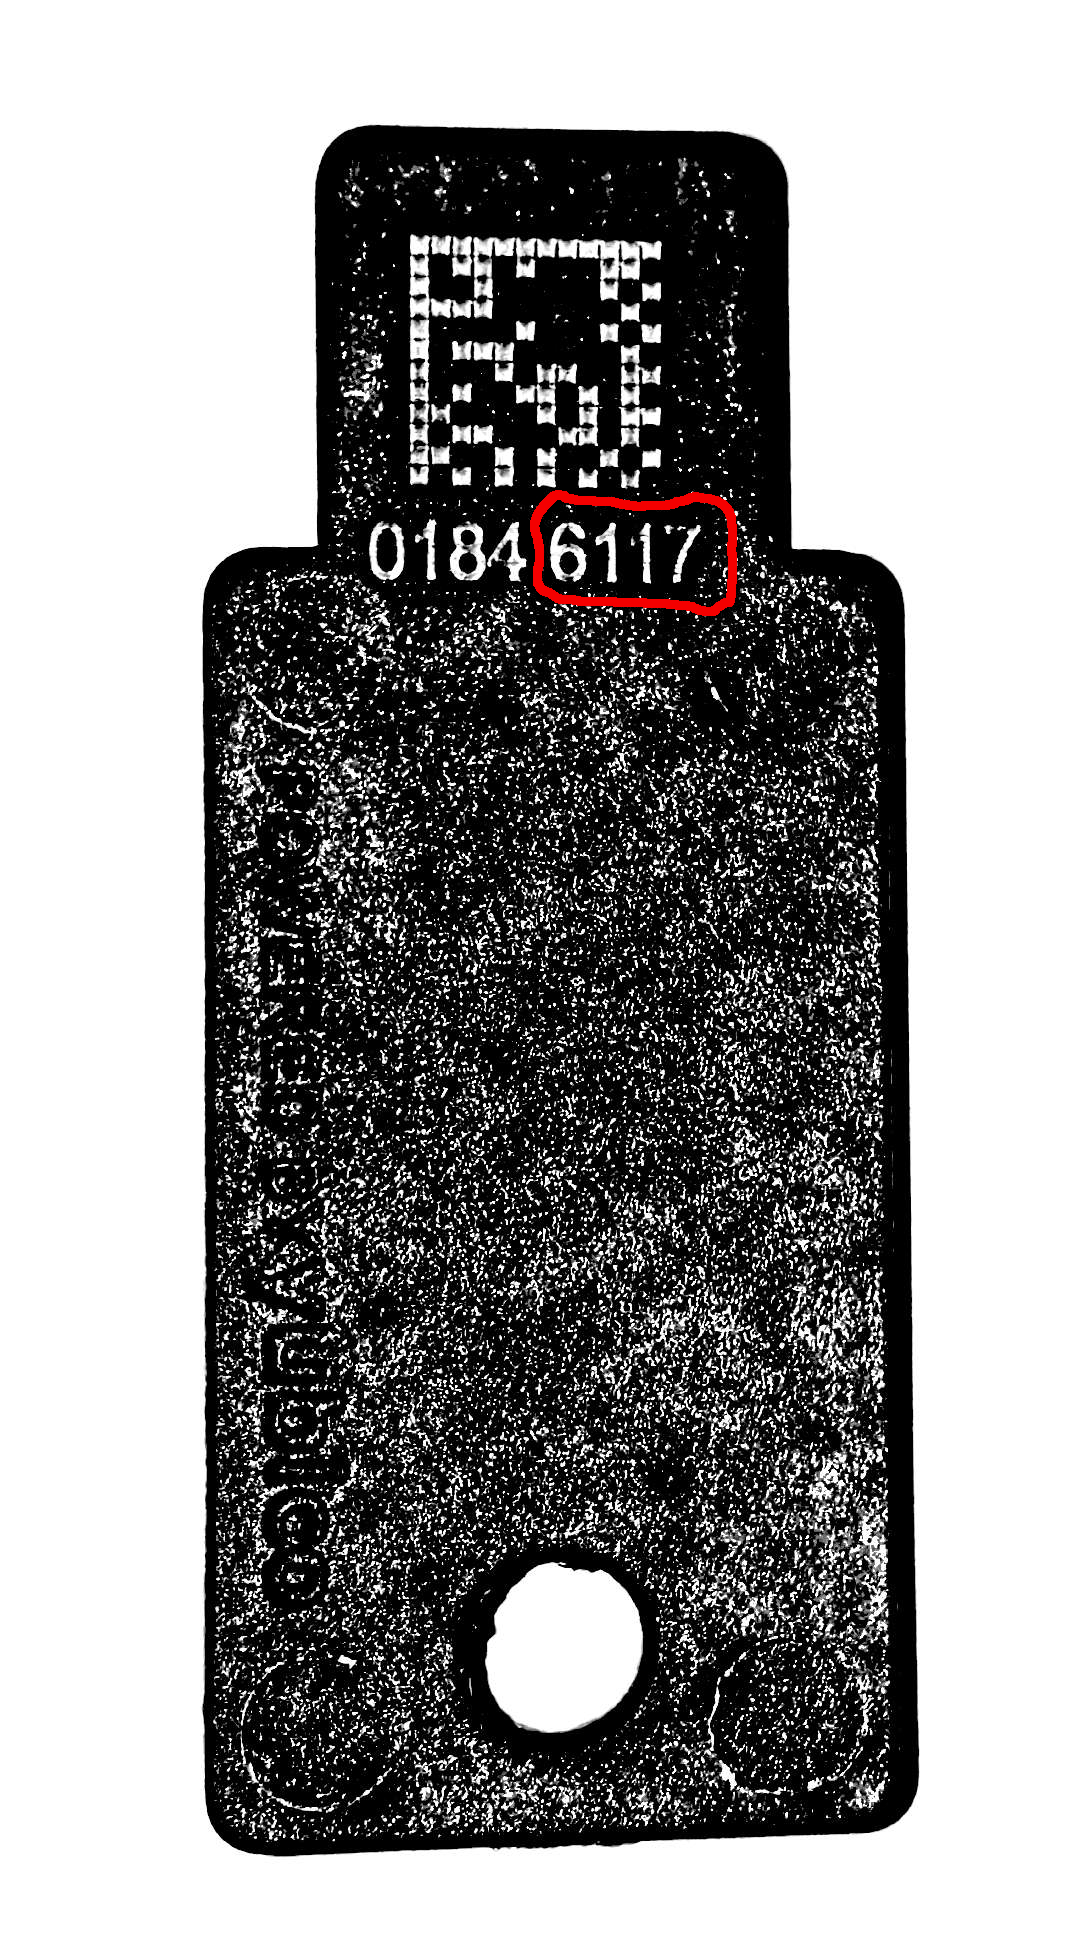
\includegraphics[width=1.5cm]{icons/yubikey1a.jpg}
    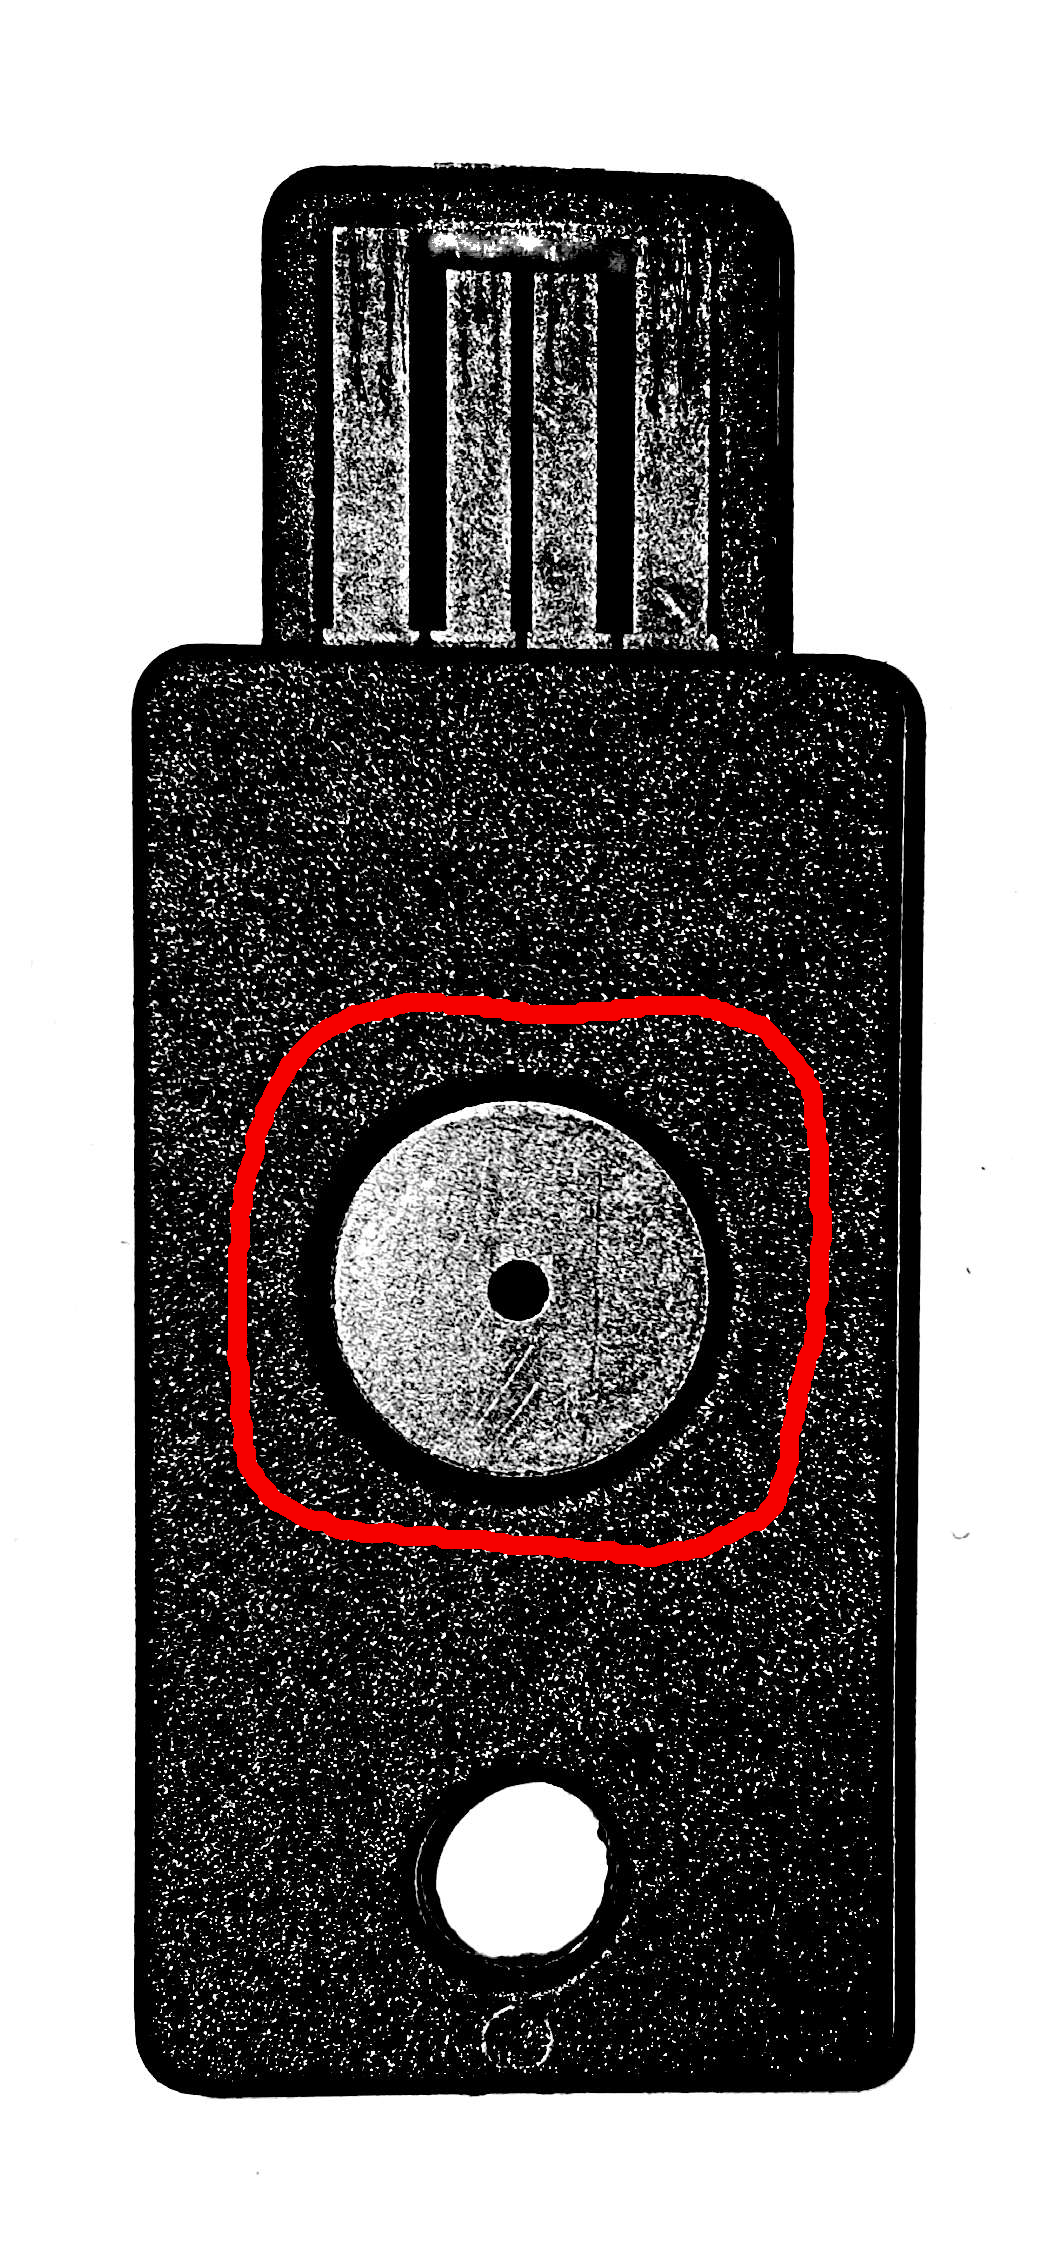
\includegraphics[width=1.3cm]{icons/yubikey2a.jpg}
    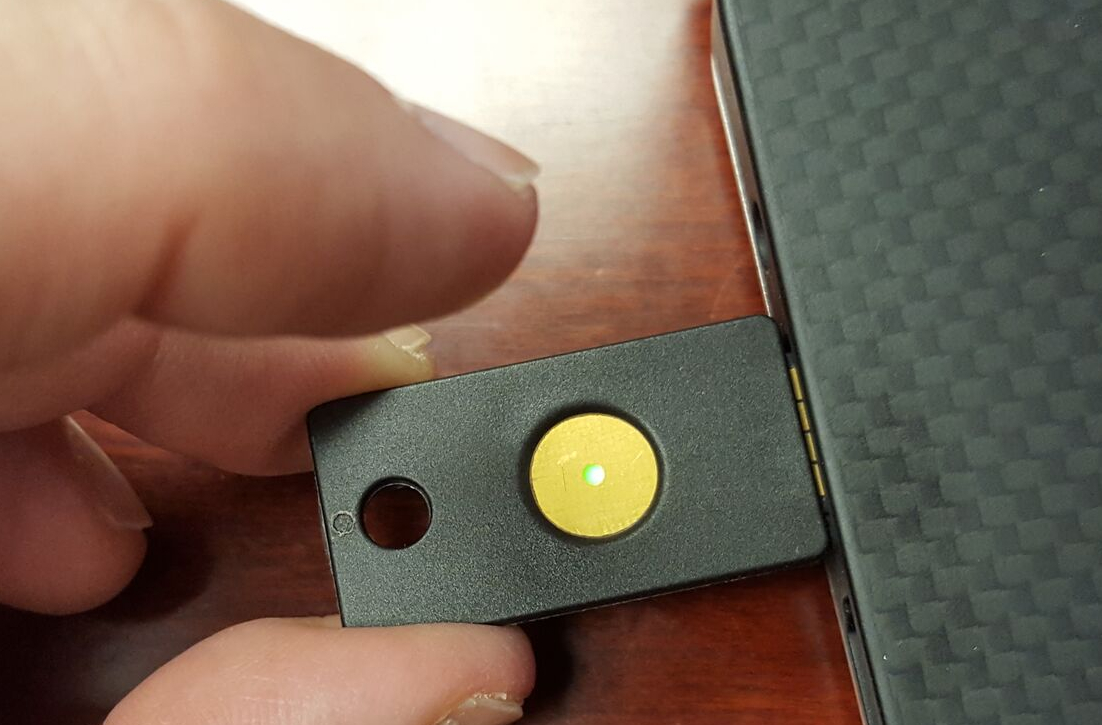
\includegraphics[width=3.3cm]{icons/yubikey3a.jpg}
  \item Use last 4 digits XXXX of yubikey as part of userid:
    {\color{mycolorcli}
\begin{verbatim}
ssh rccguest<XXXX>@midway2.rcc.uchicago.edu
\end{verbatim}
    }
  \item Push the button when asked for password
  \end{itemize}
\end{frame}

\subsection{ThinLinc}
\begin{frame}[fragile]
  \frametitle{Login to midway: ThinLinc}
  \begin{itemize}
    \item There are two ways to connect with ThinLinc to midway:
      \begin{itemize}
        \item Just use a web browser interface by pointing your browser to {\color{mycolorcli}\verb|https://midway2.rcc.uchicago.edu|}. 
          This might not work well for all browsers, you might have to try several: Chrome, Firefox, Safari...
        \item For Linux, Mac and Windows there is a client you can download from {\color{mycolorcli}\verb|https://www.cendio.com/thinlinc/download|}. 
          \begin{itemize}
          \item Configure the client to connect to {\color{mycolorcli}\verb|midway2.rcc.uchicago.edu|}
          \item You can specify the dimensions of the window in which it is running. I am usually using full screen.
          \end{itemize}
      \end{itemize}
    \item ThinLinc does not work with yubikeys, you need to have an account on midway
  \end{itemize}
\end{frame}

\documentclass{beamer}

\usepackage[utf8]{inputenc}
\usepackage{default}

\mode<presentation>
%{ \usetheme{boxes} }


\usetheme{Madrid}

\usepackage{times}
\usepackage{graphicx}
\usepackage{tabulary}
\usepackage{listings}
\usepackage{verbatimbox}
\usepackage{graphicx}
\usepackage{lmodern}
\usepackage[absolute,overlay]{textpos}
\usepackage{pgfpages}
\usepackage{color}
\usepackage{multicol}

\pgfdeclareimage[height=1.0cm]{logo_rcc}{../../../icons/logo_rcc.png}
\setlength{\TPHorizModule}{1mm}
\setlength{\TPVertModule}{1mm}
\newcommand{\RCCLogo}{
\begin{textblock}{14}(1.5,1.5)
  \pgfuseimage{logo_rcc}
\end{textblock}
}

\pgfdeclareimage[height=1.0cm]{spark}{icons/spark.png}
\newcommand{\SPARK}{
\begin{textblock}{14}(107.5,1.5)
  \pgfuseimage{spark}
\end{textblock}
}



\definecolor{mycolorcli}{RGB}{53,154,26}
\definecolor{mycolorcode}{RGB}{0,0,255}
\definecolor{mycolordef}{RGB}{255,0,0}
\definecolor{mycolorlink}{RGB}{184,4,255}

\setcounter{tocdepth}{3}

\title{\huge{Introduction to Spark}}
\author{Igor Yakushin \\ \texttt{ivy2@uchicago.edu}}

\definecolor{ChicagoMaroon}{RGB}{128,0,0}

\setbeamercolor{title}{bg=ChicagoMaroon}

\begin{document}

\setbeamertemplate{navigation symbols}{}

\setbeamercolor{fcolor}{fg=white,bg=ChicagoMaroon}
\setbeamertemplate{footline}{
\begin{beamercolorbox}[ht=4ex,leftskip=1.4cm,rightskip=.3cm]{fcolor}
\hrule
\vspace{0.1cm}
   \hfill \insertshortdate \hfill \insertframenumber/\inserttotalframenumber
\end{beamercolorbox}
}

\setbeamercolor{frametitle}{bg=ChicagoMaroon,fg=white}

\begin{frame}
\RCCLogo
\SPARK
\titlepage
\end{frame}
\section{Introduction}

\begin{frame}[fragile]
  \frametitle{Introduction}
  
\begin{itemize}
\item Apache Spark is a fast and general-purpose cluster computing system. 
\item It provides high-level APIs in Java, Scala, Python and R
\item Typically all the functionality is available in Scala and Java while APIs 
  in other languages might be behind. For example, Spark's GraphX library is only available in Scala.
\item It also supports a rich set of higher-level tools including Spark SQL for SQL 
  and structured data processing, MLlib for machine learning, GraphX for graph processing, and Spark Streaming.
\item Spark can run within Hadoop cluster and knows how to deal with various 
  Hadoop components (like HDFS, Hive, HBase, etc) and data formats.
\item Spark can also run on a standalone computer or a regular HPC cluster like midway.
\item Spark can utilize multiple nodes and multiple CPU cores in a node.
\end{itemize}

\end{frame}

\begin{frame}[fragile]
  \frametitle{Introduction}
  
  \begin{itemize}
  \item Python API, {\color{mycolordef}pyspark}, can be used 
    \begin{itemize} 
    \item in batch mode 
    \item interactively 
      \begin{itemize}
      \item in a python command prompt
      \item in Jupyter notebook
      \end{itemize}
    \end{itemize}
  \item In this tutorial we shall use only Python API to Spark mostly on midway cluster without Hadoop.
  \item The simplest way to install pyspark is to use {\color{mycolorcli}pip install pyspark}.
  \item While {\color{mycolordef}MLlib} - Spark's machine learning library -  has some Neural Network routines, for more advanced Deep Learning framework 
    consider using Spark in combination with {\color{mycolordef}BigDL} library from Intel that knows how to work with Spark's RDDs and can also be installed with
    {\color{mycolorcli}pip install bigdl}.
  \end{itemize}  
\end{frame}



\begin{frame}[fragile]
  \frametitle{Introduction}
  
\begin{itemize}
\item Spark was initially started by Matei Zaharia at UC Berkeley's AMPLab in 2009, and open sourced in 2010 under a BSD license.
\item In 2013, the project was donated to the Apache Software Foundation and switched its license to Apache 2.0. 
\item Michael Franklin, who co-founded and directed AMPLab when Spark was created, is now professor and chair at the Computer Science Department of the University of Chicago.
\item The current version of Spark is 2.3.0. 
\item We are using version 2.3.0 on midway and 2.2.0 on Hadoop cluster.
\end{itemize}
\end{frame}


\begin{frame}[fragile]
  \frametitle{Introduction}
  
\begin{itemize}
\item Before Spark 2.0, the main abstraction of Spark was the {\color{mycolordef}R}esilient {\color{mycolordef}D}istributed {\color{mycolordef}D}ataset  - {\color{mycolordef}RDD}
\item After Spark 2.0, RDD is replaced by {\color{mycolordef}DataFrame}
\item RDDs are still supported
\item It is recommended now to use {\color{mycolordef}DataFrames} instead of RDDs: 
  \begin{itemize}
  \item provides SQL interface to data - more convenient to program
  \item much faster since a query optimization, similar the one used for SQL in RDBM, is applied to queries on DataFrames but not on RDDs
  \end{itemize}
\item We shall cover both since Spark is still in the state of transition. For example:
  \begin{itemize}
    \item There are two streaming libraries: 
      \begin{itemize}
      \item {\color{mycolordef}Structured Streaming}  - based on DataFrames, 
      \item {\color{mycolordef}DStreams} - based on RDDs
      \end{itemize}
    \item There are two APIs to machine learning library: 
      \begin{itemize}
      \item the old one based on RDD is in a maintenance state - only bug fixes are applied to it but no new features are introduced; 
      \item the new machine learning library based on DataFrames is still catching up with the functionality of the old library
      \end{itemize}
  \end{itemize}
\end{itemize}

\end{frame}

\end{document}


\section{RDD}

\begin{frame}[fragile]
  \frametitle{RDD}
  
  \begin{itemize}
  \item RDD - collection of records partitioned across the nodes and can be operated on in parallel
  \item RDD can be created from files in various supported formats or by transforming other RDDs
  \item One can ask Spark to {\color{mycolordef}cache RDD in memory or disk} for fast reuse
  \item RDDs automatically recover from node failure
  \item RDD supports two types of operations:
    \begin{itemize}
    \item {\color{mycolordef}Transformations} - create a new dataset from an existing one. Lazy evaluation - evaluated only when required by action.
    \item {\color{mycolordef}Actions} - return a value to the driver program after running a computation on the dataset.
    \end{itemize}
  \end{itemize}  

\end{frame}

\subsection{Transformations}
\begin{frame}
  \frametitle{RDD: transformations}
  Examples of RDD transformations:
  \begin{itemize}
  \item {\color{mycolorcode}map(func)} - transform each element by a applying a function
  \item {\color{mycolorcode}filter(func)} - select records satisfying boolean function
  \item {\color{mycolorcode}sample(withReplacement, fraction, seed)} - Sample a fraction fraction of the data, with or without replacement, using a given random number generator seed.
  \item {\color{mycolorcode}union(otherDataset), intersection(otherDataset)}
  \item {\color{mycolorcode}distinct([numTasks]))}
  \item {\color{mycolorcode}groupByKey([numTasks])}
  \item {\color{mycolorcode}sortByKey([ascending], [numTasks])}
  \item {\color{mycolorcode}pipe(command, [envVars])}
  \end{itemize}
\end{frame}

\subsection{Actions}
\begin{frame}[fragile]
  \frametitle{RDD: actions}
  Examples of RDD actions:
  \begin{itemize}
  \item {\color{mycolorcode}reduce(func)} - Aggregate the elements of the dataset using a function func (which takes two arguments and returns one). 
    The function should be commutative and associative so that it can be computed correctly in parallel.
  \item {\color{mycolorcode}collect()} - Return all the elements of the dataset as an array at the driver program.
  \item {\color{mycolorcode}count()}
  \item {\color{mycolorcode}take(n)} - Return first n elements of the results
  \item {\color{mycolorcode}countByKey()} - Only available on RDDs of type (K, V). Returns a hashmap of (K, Int) pairs with the count of each key.
  \item {\color{mycolorcode}foreach(func)} - Run a function func on each element of the dataset. 
    This is usually done for side effects such as updating an accumulator variable (see below) or interacting with external storage systems.
  \end{itemize}
\end{frame}


\subsection{Lab 1}
\begin{frame}[fragile]
  \frametitle{RDD: Lab 1}
{\color{mycolorcode}
\begin{verbatim}
from pyspark import SparkContext, SparkConf

conf = SparkConf()
sc = SparkContext(conf=conf)

print(sc)
inputData = sc.textFile("inputFile").cache()
print(type(inputData))

numAs = inputData.filter(lambda s: 'a' in s).count()
numBs = inputData.filter(lambda s: 'b' in s).count()

print("Lines with a: %i, lines with b: %i" % (numAs, numBs))
\end{verbatim}
}

To run it:
{\color{mycolorcli}
\begin{verbatim}
make rdd
\end{verbatim}
}

\end{frame}



\section{Shared variables}
\begin{frame}
  \frametitle{Shared variables}
  \begin{itemize}
   \item Spark's second abstraction - {\color{mycolordef}shared variables}
   \item By default variables are not shared between tasks
   \item Two kinds of shared variables supported:
    \begin{itemize}
      \item {\color{mycolordef}Broadcast variables} - can be used to cache a value in memory on all nodes
      \item {\color{mycolordef}Accumulators} - such as counters, sums; one can only ``increment'' those variables; can be used to store intermediate results of reduce operation
    \end{itemize}	
  \end{itemize} 
\end{frame}

\subsection{Lab 2}
\begin{frame}[fragile]
  \frametitle{Shared variables: Lab 2}
Here we use pyspark interpreter:
{\small
{\color{mycolorcode}
\begin{verbatim}
  lines = sc.textFile("README.md")
  l1 = lines.map(lambda line: len(line.split()))
  l1.reduce(lambda a,b: a if (a>b) else b)

  pairs = lines.flatMap(lambda s: s.split()).map(lambda w: (w,1))
  result = pairs.reduceByKey(lambda a,b: a+b)
  print("\n".join(map(lambda x: "{} -> {}".format(*x), 
                      result.collect())))

  distData = sc.parallelize(list(range(1000))

  b = sc.broadcast(list(range(10)))
  b.value

  a = sc.accumulator(0)
  sc.parallelize(list(range(5))).foreach(lambda x: a.add(x))
  a.value
\end{verbatim}
}
}

\end{frame}

%\section{Spark on midway cluster}
\subsection{sinteractive}
\begin{frame}[fragile]
  \frametitle{Spark on midway cluster: sinteractive}
  \begin{itemize}
  \item So far we have seen:
    \begin{itemize}
    \item How to submit Spark job to a local node with {\color{mycolorcli}spark-submit} or {\color{mycolorcli}spark-sql}
    \item How to run pyspark locally in python interpreter
    \item How to run pyspark locally in jupyter notebook
    \end{itemize}
  \item If you are doing some heavy computations on login nodes your jobs might get killed since login nodes are not meant for it
  \item Instead you might want to grab a compute node and do the same processing there. For example:
    {\color{mycolorcli}
\begin{verbatim}
sinteractive -p broadwl --exclusive --time=3:00:00
\end{verbatim}
    }
  \item The above will give you all the cores (28) and memory (64G) on one compute node from broadwl partition for 3 hours and would allow you to work interactively.
  \item You can even run jupyter notebook on the compute nodes. For more details, see References section.
\end{itemize}
\end{frame}

\subsection{Lab7 sbatch}
\subsubsection{Single node in batch}
\begin{frame}[fragile]
  \frametitle{Spark on midway cluster: Lab 7: single node in batch}
  \begin{itemize}
  \item If you want to submit your job to a queue and run it on a single node instead of working interactively, create a batch file, {\color{mycolorcli}single.batch}
    {\color{mycolorcli}
\begin{verbatim}
#!/bin/bash

#SBATCH --job-name=single
#SBATCH --exclusive
#SBATCH --nodes=1
#SBATCH --time=00:10:00
#SBATCH --partition=broadwl
#SBATCH --output=single_%j.out
#SBATCH --error=single_%j.err
####SBATCH --account=rcc-guest

module load spark/2.3.0
export MASTER="local[*]"
spark-submit --master $MASTER perceptron.py
\end{verbatim}
    }
  \end{itemize}
\end{frame}

\begin{frame}[fragile]
  \frametitle{Spark on midway cluster: Lab 7: single node in batch}
  \begin{itemize}
  \item Notice: we are reusing perceptron example from Lab 5.
  \item To submit a job to midway
    {\color{mycolorcli}
\begin{verbatim}
sbatch single.batch
\end{verbatim}
    }
  \item To monitor the job, use
    {\color{mycolorcli}
\begin{verbatim}
squeue -j <jobid>
\end{verbatim}
    }
    or
    {\color{mycolorcli}
\begin{verbatim}
squeue -u <username>
\end{verbatim}
    }
  \item To cancel the job
    {\color{mycolorcli}
\begin{verbatim}
scancel <jobid>
\end{verbatim}
    }
  \end{itemize}
\end{frame}


\subsubsection{Multiple nodes in batch}
\begin{frame}[fragile]
  \frametitle{Spark on midway cluster: Lab 7: multiple nodes in batch}
  \begin{itemize}
  \item If you want to take advantage of using multiple nodes, 
    you have to start master Spark server on one node and slave Spark servers on the other nodes, 
    possibly including the master node. Slaves should know the address of the master.
  \item The job is submitted to the master Spark server. 
  \item To automate this procedure, {\color{mycolorcli}start-spark-slurm.sh} 
    and {\color{mycolorcli}stop-spark-slurm.sh} scripts are used.
{\color{mycolorcli}
\begin{verbatim}
...
module load spark/2.3.0

start-spark-slurm.sh

export MASTER=spark://$HOSTNAME:7077
spark-submit --master $MASTER perceptron.py

stop-spark-slurm.sh
\end{verbatim}
}

  \end{itemize}


\end{frame}


\section{Spark on Hadoop cluster}
\subsection{Batch}
\begin{frame}[fragile]
  \frametitle{Spark on Hadoop cluster: batch}
  \begin{itemize}
  \item To submit a job to a Hadoop cluster you simply need to use 
    {\color{mycolorcli}\verb|spark2-submit --master yarn <your program>.py|} on
    the login node of the Hadoop cluster
  \item Hadoop takes care of distributing the job across the nodes. You can overwrite default number of executors
    in command line arguments to {\color{mycolorcli}\verb|spark-submit|}
  \item Under Hadoop, Spark expects its input in HDFS and puts the output into HDFS
    if you use I/O-related command on RDD or DataFrame. You can still get input from local file system
    by using the full path with {\color{mycolorcli}\verb|file:///|} in front.
  \item To run {\color{mycolorcli}\verb|perceptron.py|} from Lab 7 inside Hadoop:
    {\color{mycolorcli}
\begin{verbatim}
hdfs dfs -put data
make hadoop
\end{verbatim}
    }
  \end{itemize}
\end{frame}

\subsection{Jupyter}
\begin{frame}[fragile]
  \frametitle{Spark on Hadoop cluster: jupyter}
\begin{itemize}
\item Point your browser to
{\color{mycolorcli}
\begin{verbatim}
https://hadoop.rcc.uchicago.edu/
\end{verbatim}
}
\item Login using your midway credentials.
\item Browse into {\color{mycolorcli}\verb|Spark/labs/3|} and open {\color{mycolorcli}\verb|lab3.ipynb|}
\item Change the kernel to {\color{mycolorcli}\verb|pySpark 2.2.0|}: \verb|Kernel -> Change Kernel -> pySpark 2.2.0|
\item One can execute a cell in the notebook with Shift+Enter.
\item The main thing to remember: unless you shut down the notebook, it continues running and using Hadoop resources even if you
  close the browser and turn off your computer!!! As a result, the next user might not be able to get access to Spark either
  from jupyter or even in batch. This happens especially often at the end of the semester when students are doing the final project.
  There is a script running killing pyspark jobs that have been running for more than 3 hours.
\end{itemize}
\end{frame}

\begin{frame}[fragile]
  \frametitle{Spark on Hadoop cluster: jupyter}

Two ways to shut down a jupyter notebook:

\begin{itemize}
\item When inside the notebook: \verb|File -> Close and Halt|
\item When in the file browser outside of the notebook: select ``Running'' tab and press the yellow ``Shutdown'' button near
  any running notebook.
\end{itemize}
\end{frame}
\section{Spark SQL}

\begin{frame}[fragile]
  \frametitle{Spark SQL}
  
  \begin{itemize}
  \item {\color{mycolordef}Spark SQL} is a component on top of Spark that introduced a data abstraction called {\color{mycolordef}DataFrames}, which provides support for structured and semi-structured data. 
  \item DataFrame is like a table distributed over the cluster similar to RDD
  \item One can query DataFrame using 
    \begin{itemize}
    \item Spark language
    \item SQL - language for queries on relational databases
    \end{itemize}
  \item In both cases the query optimization is used that typically results in a better performance over RDDs
  \item One can create DataFrame by applying transformations to other DataFrames, from the same sources as RDD: RDD, text files, json files, arrays, files in various Hadoop formats like parquet.
  \item Spark SQL can be interfaced with relational databases via ODBC/JDBC
  \item Spark SQL can use distributed Thrift store via ODBC/JDBC
  \item Spark SQL can use Hive store
  \end{itemize}
\end{frame}

\subsection{Lab 1}
\subsubsection{line\_count\_DF.py}
\begin{frame}[fragile]
  \frametitle{Spark SQL: Lab 1}
{\small
{\color{mycolorcode}
\begin{verbatim}
from pyspark import SparkContext, SparkConf
from pyspark.sql import SparkSession

sc = SparkContext(conf=SparkConf())
spark = SparkSession(sc)

inputData = spark.read.text(inputFile).cache()

numAs = inputData.filter(inputData.value.contains('a')).count()
numBs = inputData.filter(inputData.value.contains('b')).count()

print("Lines with a: %i, lines with b: %i" % (numAs, numBs))
\end{verbatim}
}
}
\end{frame}

\subsection{Lab 3}
\subsubsection{lab3.ipynb}
\begin{frame}[fragile]
  \frametitle{Spark SQL: Lab 3: lab3.ipynb}
  We use jupyter notebook:
{\color{mycolorcode}
\begin{verbatim}
lines = spark.read.text("README.md") 
from pyspark.sql.functions import *
z=lines.select(explode(split(lines.value,"\s+")).name("w"))
z.groupBy("w").count().take(10)
\end{verbatim}
}
\end{frame}


\subsection{Lab 4}
\subsubsection{sql.py}
\begin{frame}[fragile]
  \frametitle{Spark SQL: Lab 4: sql.py}
{\color{mycolorcode}
\begin{verbatim}
js = "data/people.json"
df = spark.read.json(js)
df.show()
df.printSchema()
df.select("name").show()
df.select(df['name'], df['age'] + 1).show()
df.filter(df['age'] > 21).show()
df.groupBy("age").count().show()

df.createOrReplaceTempView("people")
sqlDF = spark.sql("SELECT * FROM people")
sqlDF.show()
\end{verbatim}
}
\end{frame}

\subsubsection{rdd2df.py}
\begin{frame}[fragile]
  \frametitle{Spark SQL: Lab 4: rdd2df.py}
{\small
{\color{mycolorcode}
\begin{verbatim}
from pyspark.sql import SparkSession
from pyspark.sql import Row

spark = SparkSession.builder.getOrCreate()
sc = spark.sparkContext

lines = sc.textFile("data/people.txt")
parts = lines.map(lambda l: l.split(","))
people = parts.map(lambda p: Row(name=p[0], age=int(p[1])))

schemaPeople = spark.createDataFrame(people)
schemaPeople.createOrReplaceTempView("people")
teens = spark.sql("SELECT name FROM people 
                   WHERE age >= 13 AND age <= 19")
teenNames = teens.rdd.map(lambda p: "Name: " + p.name).collect()
for name in teenNames:
    print(name)
\end{verbatim}
}
}
\end{frame}

\subsubsection{files.py}
\begin{frame}[fragile]
  \frametitle{Spark SQL: Lab 4: files.py}
{\small
{\color{mycolorcode}
\begin{verbatim}
from pyspark.sql import SparkSession
from os.path import abspath
warehouse_location = abspath('spark-warehouse')
spark = SparkSession \
    .builder \
    .appName("Python Spark SQL Hive integration example") \
    .config("spark.sql.warehouse.dir", warehouse_location) \
    .enableHiveSupport() \
    .getOrCreate()
df = spark.read.load("data/users.parquet")
df.select("name", "favorite_color").write.save("output/t.parquet")

df = spark.sql("SELECT * FROM parquet.`data/users.parquet`")
print(df.show())

df.write.saveAsTable("users1")
df.write.option("path", "output/hive").saveAsTable("users")
\end{verbatim}
}
}
\end{frame}



\subsubsection{hive.py}
\begin{frame}[fragile]
  \frametitle{Spark SQL: Lab 4: hive.py}
{\small
{\color{mycolorcode}
\begin{verbatim}
warehouse_location = abspath('spark-warehouse')
spark = SparkSession \
    .builder \
    .appName("Python Spark SQL Hive integration example") \
    .config("spark.sql.warehouse.dir", warehouse_location) \
    .enableHiveSupport() \
    .getOrCreate()
spark.sql("CREATE TABLE IF NOT EXISTS 
           src (key INT, value STRING) USING hive")
spark.sql("LOAD DATA LOCAL INPATH 
           'data/kv1.txt' INTO TABLE src")
spark.sql("SELECT * FROM src").show()

spark.sql("SELECT * FROM users1").show()
\end{verbatim}
}
}
\end{frame}


\subsubsection{hive.sql}
\begin{frame}[fragile]
\frametitle{Spark SQL: Lab 4: hive.sql}
\begin{itemize}
\item hive.sql:
{\small
{\color{mycolorcode}
\begin{verbatim}
select * from users1;
\end{verbatim}
}
}

\item spark-sql:
{\small
{\color{mycolorcli}
\begin{verbatim}
spark-sql --master local[1] --name "spark-sql example" 
          -f hive.sql 1>spark_sql.out 2>spark_sql.err
\end{verbatim}
}
}
\end{itemize}
\end{frame}

\section{Machine Learning Library}
\subsubsection{hive.sql}
\begin{frame}[fragile]
\frametitle{Machine Learning Library}
\begin{itemize}
\item Spark Machine Learning Library - {\color{mycolordef}MLlib} - is a distributed machine learning framework on top of Spark
\item MLlib has RDD and DataFrame APIs
\item RDD API is now in maintenance mode: bugs are fixed, no new features are added
\item DataFrame API is catching up, once it does, RDD API will be removed
\item Many common machine learning and statistical algorithms have been implemented and are shipped with MLlib which simplify large scale machine learning pipelines, including:
  \begin{itemize}
    \item summary statistics, correlations, sampling, hypothesis testing
    \item classification and regression: support vector machines, logistic regression, linear regression, decision trees, naive Bayes classification
    \item cluster analysis methods including k-means
    \item dimensionality reduction techniques such as SVD and PCA
    \item feature extraction and transformation functions
    \item optimization algorithms such as stochastic gradient descent
  \end{itemize}
\end{itemize}
\end{frame}

\subsection{Lab 5}
\subsubsection{Logistic Regression}
\begin{frame}[fragile]
\frametitle{Lab 5: Logistic Regression}
\begin{itemize}
\item In this lab we have a training set consisting of class label (0 or 1) and 692 numerical features
\item The data is sparse and is given in libsvm format in {\color{mycolorcli}\verb|data/sample_libsvm_data.txt|}
\item Linear regression model tries to predict the class $y$ based on features 
  $x_i$ as follows:
  \begin{equation*}
    y = \frac{1}{1 + e^{-(\sum_{i}{w_i x_i} + b)}} 
  \end{equation*}
  where $w_i$ and $b$ are parameters that the model needs to learn to minimize error on the given training set. 
  \item After the model is trained, the parameters are printed. 
  \item Since most of them are zero, sparse format is used.
\end{itemize}
\end{frame}


\begin{frame}[fragile]
\frametitle{Lab 5: Logistic Regression}
{\small
{\color{mycolorcode}
\begin{verbatim}
from pyspark.sql import SparkSession
from pyspark.ml.classification import LogisticRegression

spark = SparkSession.builder.getOrCreate()

# Load training data
training = spark.read.format("libsvm").\
                 load("data/sample_libsvm_data.txt")
lr = LogisticRegression(maxIter=10, 
                   regParam=0.3, elasticNetParam=0.8)
# Fit the model
lrModel = lr.fit(training)

# Print the coefficients and intercept for logistic regression
print("Coefficients: " + str(lrModel.coefficients))
print("Intercept: " + str(lrModel.intercept))
\end{verbatim}
}
}
\end{frame}

\subsubsection{Perceptron}
\begin{frame}[fragile]
\frametitle{Lab 5: Perceptron}
\begin{columns}
\begin{column}{.75\textwidth}
\begin{itemize}
\item The data has 3 classes and 4 features and is given in libsvm format 
  {\small{\color{mycolorcli}\verb|data/sample_multiclass_classification_data.txt|}}
\item The model is a fully connected neural network with 4 layers.
\item \verb|60%| of data is used as training set and \verb|40%| as validation set.
\item 100 epochs is used for training, mini-batch size is 128.
\item Prediction accuracy on the validation set is printed: \verb|90%|.
\end{itemize}
\end{column}

\begin{column}{.25\textwidth}
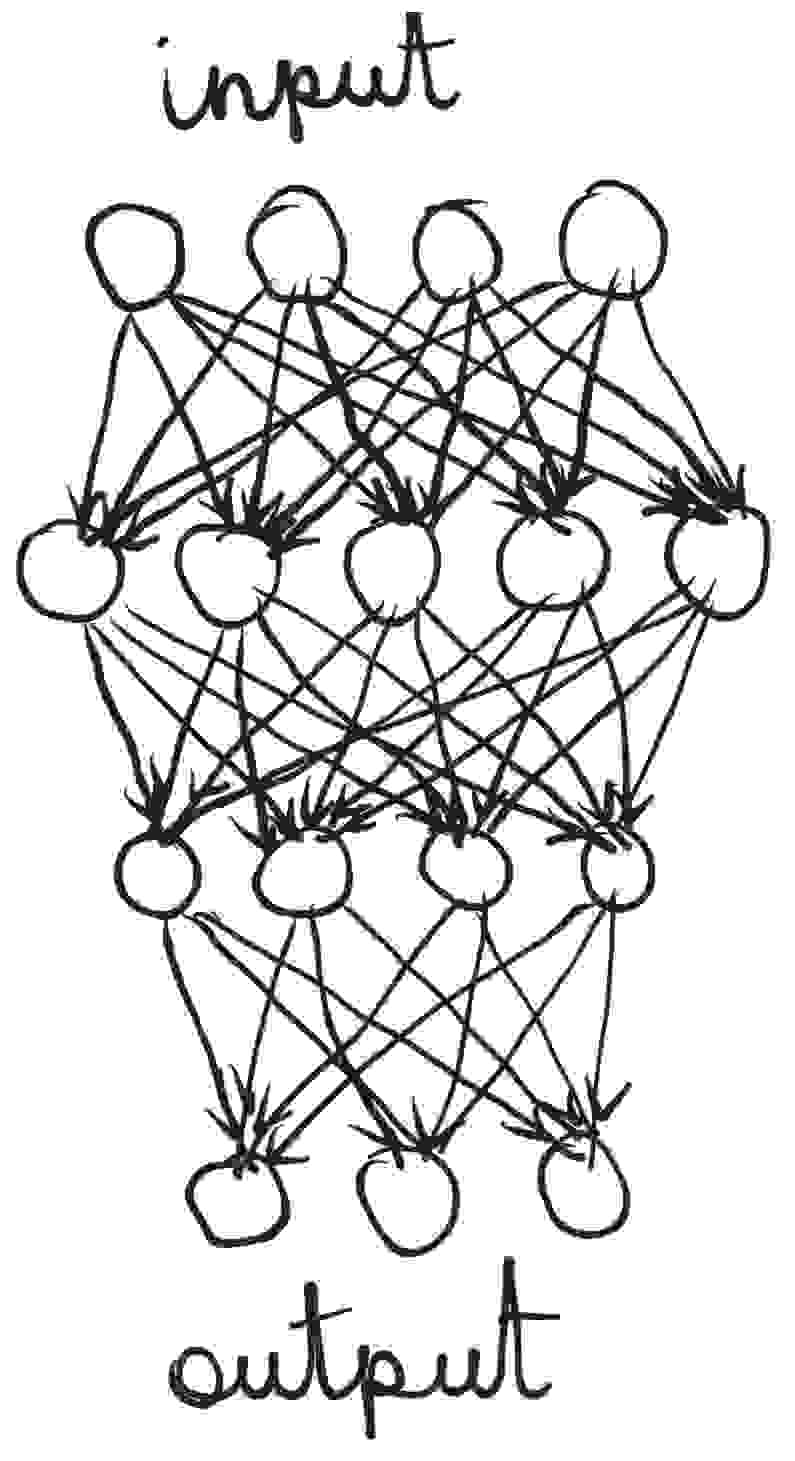
\includegraphics[width=3cm]{graphs/perceptron.jpg}
\end{column}


\end{columns}

\end{frame}


\begin{frame}[fragile]
\frametitle{Lab 5: Perceptron}
{\small
{\color{mycolorcode}
\begin{verbatim}
from pyspark.ml.classification 
     import MultilayerPerceptronClassifier as mlp
from pyspark.ml.evaluation 
     import MulticlassClassificationEvaluator as mce
spark = SparkSession.builder.getOrCreate()
data = spark.read.format("libsvm")\
    .load("data/sample_multiclass_classification_data.txt")
splits = data.randomSplit([0.6, 0.4], 1234)
train = splits[0]; test = splits[1]
layers = [4, 5, 4, 3]
trainer = mlp(maxIter=100, layers=layers, blockSize=128, seed=1234)
model = trainer.fit(train)
result = model.transform(test)
predictionAndLabels = result.select("prediction", "label")
evaluator = mce(metricName="accuracy")
print(evaluator.evaluate(predictionAndLabels))))
\end{verbatim}
}
}
\end{frame}

\section{Streaming}
\begin{frame}[fragile]
\frametitle{Streaming}
\begin{itemize}
\item Streaming allows to process continuously arriving data
\item There are two streaming interfaces in Spark:
  \begin{itemize}
  \item {\color{mycolordef}Structured Streaming} - DataFrame API
  \item {\color{mycolordef}Spark Streaming (DStreams)} - RDD API
  \end{itemize}
\item We shall only consider Structured Streaming.
\item Structured Streaming is a scalable and fault-tolerant stream processing engine built on the Spark SQL engine. 
\item One can express streaming computation the same way one would express a batch computation on static data. 
\item The Spark SQL engine will take care of running it incrementally and continuously and updating the final result as streaming data continues to arrive
\item Structured Streaming can use as sources: files, Kafka, socket (for testing)
\end{itemize}
\end{frame}

\subsection{Lab 6}
\subsubsection{word\_count.py}
\begin{frame}[fragile]
\frametitle{Streaming: Lab 6: word\_count.py}
{\small
{\color{mycolorcode}
\begin{verbatim}
from pyspark.sql.functions import explode, split
import sys
port = int(sys.argv[1]); host = sys.argv[2]
spark = SparkSession.builder.getOrCreate()
lines = spark.readStream.format("socket") \
    .option("host",host).option("port",port).load()
words = lines.select(
   explode(
       split(lines.value, " ")
   ).alias("word")
)
wordCounts = words.groupBy("word").count()
query = wordCounts \
    .writeStream \
    .outputMode("complete") \
    .format("console") \
    .start()
query.awaitTermination()
\end{verbatim}
}}
\end{frame}

\begin{frame}[fragile]
\frametitle{Streaming: Lab 6: word\_count.py}
\begin{itemize}
\item Generate random port number from 9000 to 10000 and write the corresponding commands used below into the files 
  {\color{mycolorcli}mync.sh} and {\color{mycolorcli}mystream.sh}.
\item Open the second terminal on the same host and run {\color{mycolorcli}netcat} in it:
{\color{mycolorcli}
\begin{verbatim}
source env.sh
make nc
\end{verbatim}
}
\item netcat will connect to {\color{mycolorcli}\verb|localhost:<port>|}
\item In the first terminal, start pyspark streaming program:
{\color{mycolorcli}
\begin{verbatim}
make word_count
\end{verbatim}
}
\item Now pyspark listens to input on {\color{mycolorcli}\verb|localhost:<port>|}
\item In the second terminal type some words. Once you hit {\color{mycolorcli}Enter}, 
  all the words including the current ones are reprocessed by pyspark. 
  Keep entering new lines and observe the output in the first terminal.
\item To stop both processes, type {\color{mycolorcli}Ctrl+C} in the window with pyspark.
\end{itemize}
\end{frame}

\subsubsection{age.py}
\begin{frame}[fragile]
\frametitle{Streaming: Lab 6: age.py}
{\small
{\color{mycolorcode}
\begin{verbatim}
from pyspark.sql import SparkSession
from pyspark.sql.types import StructType
from pyspark.sql.functions import avg

spark = SparkSession.builder.getOrCreate()

userSchema = StructType().add("name", "string")\
                         .add("age", "integer")
csvDF = spark.readStream.option("sep", ";") \
    .schema(userSchema).csv("input_csv")

averageAge = csvDF.select(avg(csvDF.age))

query = averageAge.writeStream.outputMode("complete")\
                              .format("console").start()
query.awaitTermination()
\end{verbatim}
}
}
\end{frame}

\begin{frame}[fragile]
\frametitle{Streaming: Lab 6: age.py}
\begin{itemize}
\item In this lab data is processed as files are added into {\color{mycolorcli}\verb|input_csv|} directory
\item First start pyspark by running
{\color{mycolorcli}
\begin{verbatim}
make age
\end{verbatim}
}
\item In the second terminal 
{\color{mycolorcli}
\begin{verbatim}
mv tmp/1.csv input_csv/
\end{verbatim}
}
\item Observe average age computed in the first terminal
\item Next
{\color{mycolorcli}
\begin{verbatim}
mv tmp/2.csv input_csv/
\end{verbatim}
}
\item Notice: it is important to use {\color{mycolorcli}mv} because files for Spark Streaming are supposed to be immutable. {\color{mycolorcli}mv} simply renames a file instantaneously while 
something like {\color{mycolorcli}cp} might take time. As a result Spark might process the first part of the file it notices and ignore the rest.
\end{itemize}
\end{frame}


\section{Spark on midway cluster}
\subsection{sinteractive}
\begin{frame}[fragile]
  \frametitle{Spark on midway cluster: sinteractive}
  \begin{itemize}
  \item So far we have seen:
    \begin{itemize}
    \item How to submit Spark job to a local node with {\color{mycolorcli}spark-submit} or {\color{mycolorcli}spark-sql}
    \item How to run pyspark locally in python interpreter
    \item How to run pyspark locally in jupyter notebook
    \end{itemize}
  \item If you are doing some heavy computations on login nodes your jobs might get killed since login nodes are not meant for it
  \item Instead you might want to grab a compute node and do the same processing there. For example:
    {\color{mycolorcli}
\begin{verbatim}
sinteractive -p broadwl --exclusive --time=3:00:00
\end{verbatim}
    }
  \item The above will give you all the cores (28) and memory (64G) on one compute node from broadwl partition for 3 hours and would allow you to work interactively.
  \item You can even run jupyter notebook on the compute nodes. For more details, see References section.
\end{itemize}
\end{frame}

\subsection{Lab7 sbatch}
\subsubsection{Single node in batch}
\begin{frame}[fragile]
  \frametitle{Spark on midway cluster: Lab 7: single node in batch}
  \begin{itemize}
  \item If you want to submit your job to a queue and run it on a single node instead of working interactively, create a batch file, {\color{mycolorcli}single.batch}
    {\color{mycolorcli}
\begin{verbatim}
#!/bin/bash

#SBATCH --job-name=single
#SBATCH --exclusive
#SBATCH --nodes=1
#SBATCH --time=00:10:00
#SBATCH --partition=broadwl
#SBATCH --output=single_%j.out
#SBATCH --error=single_%j.err
####SBATCH --account=rcc-guest

module load spark/2.3.0
export MASTER="local[*]"
spark-submit --master $MASTER perceptron.py
\end{verbatim}
    }
  \end{itemize}
\end{frame}

\begin{frame}[fragile]
  \frametitle{Spark on midway cluster: Lab 7: single node in batch}
  \begin{itemize}
  \item Notice: we are reusing perceptron example from Lab 5.
  \item To submit a job to midway
    {\color{mycolorcli}
\begin{verbatim}
sbatch single.batch
\end{verbatim}
    }
  \item To monitor the job, use
    {\color{mycolorcli}
\begin{verbatim}
squeue -j <jobid>
\end{verbatim}
    }
    or
    {\color{mycolorcli}
\begin{verbatim}
squeue -u <username>
\end{verbatim}
    }
  \item To cancel the job
    {\color{mycolorcli}
\begin{verbatim}
scancel <jobid>
\end{verbatim}
    }
  \end{itemize}
\end{frame}


\subsubsection{Multiple nodes in batch}
\begin{frame}[fragile]
  \frametitle{Spark on midway cluster: Lab 7: multiple nodes in batch}
  \begin{itemize}
  \item If you want to take advantage of using multiple nodes, 
    you have to start master Spark server on one node and slave Spark servers on the other nodes, 
    possibly including the master node. Slaves should know the address of the master.
  \item The job is submitted to the master Spark server. 
  \item To automate this procedure, {\color{mycolorcli}start-spark-slurm.sh} 
    and {\color{mycolorcli}stop-spark-slurm.sh} scripts are used.
{\color{mycolorcli}
\begin{verbatim}
...
module load spark/2.3.0

start-spark-slurm.sh

export MASTER=spark://$HOSTNAME:7077
spark-submit --master $MASTER perceptron.py

stop-spark-slurm.sh
\end{verbatim}
}

  \end{itemize}


\end{frame}


\section{Spark on Hadoop cluster}
\subsection{Batch}
\begin{frame}[fragile]
  \frametitle{Spark on Hadoop cluster: batch}
  \begin{itemize}
  \item To submit a job to a Hadoop cluster you simply need to use 
    {\color{mycolorcli}\verb|spark2-submit --master yarn <your program>.py|} on
    the login node of the Hadoop cluster
  \item Hadoop takes care of distributing the job across the nodes. You can overwrite default number of executors
    in command line arguments to {\color{mycolorcli}\verb|spark-submit|}
  \item Under Hadoop, Spark expects its input in HDFS and puts the output into HDFS
    if you use I/O-related command on RDD or DataFrame. You can still get input from local file system
    by using the full path with {\color{mycolorcli}\verb|file:///|} in front.
  \item To run {\color{mycolorcli}\verb|perceptron.py|} from Lab 7 inside Hadoop:
    {\color{mycolorcli}
\begin{verbatim}
hdfs dfs -put data
make hadoop
\end{verbatim}
    }
  \end{itemize}
\end{frame}

\subsection{Jupyter}
\begin{frame}[fragile]
  \frametitle{Spark on Hadoop cluster: jupyter}
\begin{itemize}
\item Point your browser to
{\color{mycolorcli}
\begin{verbatim}
https://hadoop.rcc.uchicago.edu/
\end{verbatim}
}
\item Login using your midway credentials.
\item Browse into {\color{mycolorcli}\verb|Spark/labs/3|} and open {\color{mycolorcli}\verb|lab3.ipynb|}
\item Change the kernel to {\color{mycolorcli}\verb|pySpark 2.2.0|}: \verb|Kernel -> Change Kernel -> pySpark 2.2.0|
\item One can execute a cell in the notebook with Shift+Enter.
\item The main thing to remember: unless you shut down the notebook, it continues running and using Hadoop resources even if you
  close the browser and turn off your computer!!! As a result, the next user might not be able to get access to Spark either
  from jupyter or even in batch. This happens especially often at the end of the semester when students are doing the final project.
  There is a script running killing pyspark jobs that have been running for more than 3 hours.
\end{itemize}
\end{frame}

\begin{frame}[fragile]
  \frametitle{Spark on Hadoop cluster: jupyter}

Two ways to shut down a jupyter notebook:

\begin{itemize}
\item When inside the notebook: \verb|File -> Close and Halt|
\item When in the file browser outside of the notebook: select ``Running'' tab and press the yellow ``Shutdown'' button near
  any running notebook.
\end{itemize}
\end{frame}
\section{BigDL}

\begin{frame}[fragile]
  \frametitle{BigDL}
  \begin{itemize}
  \item {\color{mycolordef}BigDL} is a library for Deep Learning from Intel
  \item It is fully integrated with Spark and can work directly with RDDs
  \item While MLlib has some machine learning algorithms, 
    including fully connected Neural Networks, it does not currently implement Deep Learning models
  \item BigDL runs on CPU only and relies on MKL for multithreading
  \item The installation of python version of BigDL is as simple as 
    {\color{mycolorcli}
\begin{verbatim}
pip install BigDL
\end{verbatim}
    }
  \item BigDL API appears to be very similar to Keras
  \end{itemize}
\end{frame}


\subsection{Lab 8}
\begin{frame}[fragile]
  \frametitle{BigDL: Lab 8}
  \begin{itemize}
  \item In this lab we use the models supplied with BigDL
  \item {\color{mycolorcli}\verb|local_lenet.py|} is a standalone (no Spark) 
    BigDL program to train LeNet model for handwritten digits recognition
  \item Run it on a single compute node with
    {\color{mycolorcli}
\begin{verbatim}
make lenet_local
\end{verbatim}
    }
  \item {\color{mycolorcli}lenet5.py} is using both Spark and BigDL.
  \item Run it on a single compute node with
    {\color{mycolorcli}
\begin{verbatim}
make lenet5
\end{verbatim}
    }
\end{itemize}
\end{frame}


\begin{frame}[fragile]
  \frametitle{BigDL: Lab 8}
  \begin{itemize}
  \item LeNet has been used for decades by USPS to recognize handwritten zip codes
  \item Here is how LeNet model is built in BigDL:
{\small
    {\color{mycolorcode}
\begin{verbatim}
def build_model(class_num):
    model = Sequential()
    model.add(Reshape([1, 28, 28]))
    model.add(SpatialConvolution(1, 6, 5, 5))
    model.add(Tanh())
    model.add(SpatialMaxPooling(2, 2, 2, 2))
    model.add(Tanh())
    model.add(SpatialConvolution(6, 12, 5, 5))
    model.add(SpatialMaxPooling(2, 2, 2, 2))
    model.add(Reshape([12 * 4 * 4]))
    model.add(Linear(12 * 4 * 4, 100))
    model.add(Tanh())
    model.add(Linear(100, class_num))
    model.add(LogSoftMax())
    return model
\end{verbatim}
    }
}
\end{itemize}
\end{frame}


\begin{frame}[fragile]
  \frametitle{BigDL: Lab 8}
  \begin{itemize}
  \item MNIST data is loaded into RDD and is preprocessed in Spark before going into BigDL:
{\small
    {\color{mycolorcode}
\begin{verbatim}
train_data = get_mnist(sc, "train", options.dataPath)\
     .map(lambda rec_tuple: (normalizer(rec_tuple[0],\
      mnist.TRAIN_MEAN, mnist.TRAIN_STD), rec_tuple[1]))\
     .map(lambda t: Sample.from_ndarray(t[0], t[1]))
\end{verbatim}
}
}
\end{itemize}
\end{frame}


\section{Conclusion}
\begin{frame}[fragile]
  \frametitle{Conclusion}
  \begin{itemize}
  \item In this tutorial we covered Python API to Spark:
    \begin{itemize}
    \item Spark Core: RDDs, shared variables
    \item Spark SQL: DataFrames
    \item Spark Machine Learning Library
    \item Spark Streaming
    \end{itemize}
  \item We also briefly looked into integrating Spark with BigDL library for Deep Learning
  \item We have not looked into Scala, Java and R Spark APIs
  \item We also have not discussed GraphX library since so far it is only implemented in Scala
  \item We learned how to run Spark on a local computer, on general purpose cluster under Slurm and on Hadoop cluster under Yarn
  \item We learned how to use Spark in batch or interactively in python shell or jupyter notebook
  \end{itemize}
\end{frame}
\section{References}

\begin{frame}[fragile]
  \frametitle{References}

{\tiny
\begin{verbatim}
Apache Spark home page:
https://spark.apache.org

How Companies are Using Spark, and Where the Edge in Big Data Will Be
by Matei Zaharia
https://conferences.oreilly.com/strata/strata2014/public/schedule/detail/33057

Deep Learning Tutorials on Apache Spark using BigDL
https://github.com/intel-analytics/BigDL-Tutorials

Running Jupyter on a midway compute node
https://git.rcc.uchicago.edu/ivy2/Jupyter_on_compute_nodes

Troubleshooting JupyterHub and jupyter notebook
https://git.rcc.uchicago.edu/ivy2/Troubleshooting_JupyterHub

Introduction to Hadoop
https://git.rcc.uchicago.edu/ivy2/Graham_Introduction_to_Hadoop
\end{verbatim}
}

\end{frame}
\section{Appendix: tutorials on demand}
\begin{frame}[fragile]
  \frametitle{Tutorials on demand}
  \begin{itemize}
    \item I accept requests for doing tutorials on demand, outside of regular RCC Workshops schedule
    \item The tutorials can also be integrated into regular courses. For example, last year I did 
      \begin{itemize}
      \item ``Distributed MPI Programming in Python'' as part of the ``Computational Astrophysics'' course for graduate students
      \item ``Deep Learning with Keras'' as part of the ``Computational Physics'' course for undergraduate students
      \end{itemize}
    \item Currently the following tutorials are available at any time:
      \begin{itemize}
        \item Distributed MPI programming in C/C++/Python
        \item Introduction to Linux and RCC
        \item Introduction to Python
        \item Introduction to Hadoop
        \item Deep Learning with Keras and TensorFlow
        \item Deep Learning with Theano
        \item Singularity Container
        \item Introduction to Spark
      \end{itemize}
    \item More are coming soon...
  \end{itemize}
\end{frame}

\end{document}

